
在我们已经了解过的顺序数据结构中,数据都存储在一个数组中(或者是一个由内存块组成的数组)。现在我们将考虑一种不同类型的数据结构,其中数据是通过指针连接在一起的。最简单的例子就是一个链表,其中每个元素都是单独分配的,这里了解到的方法也适用于其他节点容器,如树、图或其他数据结构,其中每个元素都是单独分配的,数据通过指针连接在一起。

为了简单起见,我们先来看一个单链表。在STL中,为\texttt{std::forward\_list}:

%\hspace*{\fill} \\ %插入空行
\begin{center}
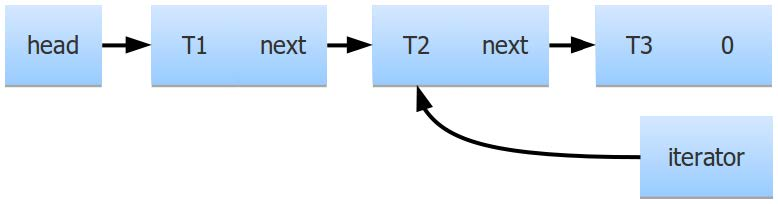
\includegraphics[width=0.9\textwidth]{content/2/chapter7/images/24.jpg}\\
图7.24 - 带有迭代器的单链表
\end{center}

因为每个元素都是单独分配的,所以也可以单独回收。通常,轻量级分配器用于这些数据结构,其中内存在大块中分配,这些大块划分为节点大小的片段。当一个节点释放时,内存不会返回给操作系统,而是放在一个空闲列表中,以便应对下一次分配内存的请求。就我们的目的而言,内存直接从操作系统分配,还由专门的分配器处理,与我们的关系不大(后者通常更高效)。

并发程序中,链表的迭代器是一个挑战。如图7.24,这些迭代器可以指向链表中的任何位置。如果有元素从列表中删除,则希望它的内存能够用于构造和插入另一个元素(如果不这样做,并保持所有内存直到整个列表删除,重复增加和删除元素会浪费大量的内存)。但是,如果有指向链表节点的迭代器,则不能删除该节点。在单线程程序中也是如此,但是在并发程序中的管理通常要困难得多。对于可能使用多个线程的迭代器,通常不能通过操作的执行流保证没有迭代器指向要删除的元素。本例中,需要迭代器来扩展它们所指向的链表节点的生命周期。当然,这是一个使用引用计数的智能指针的工作,比如\texttt{std::shared\_ptr}。现在,我们假设链表中的所有指针,包括连接节点和迭代器中的指针,都是智能指针(\texttt{std::shared\_ptr}或类似的具有强线程安全保证的指针)。

就像处理顺序数据结构一样,对线程安全的数据结构的第一次尝试应该是使用锁保护的实现。在确定需要之前,永远不要设计无锁数据结构:开发无锁代码可能很酷,但试图在其中找到bug则很困难。

就像前做的那样,我们必须重新设计部分接口,所有的操作都是事务性的:例如,\texttt{pop\_front()}应该工作,无论链表是否为空。然后,可以用锁保护所有操作。对于\texttt{push\_front()}和\textbf{}pop\_front()}这样的操作,很可能类似于之前观察到的堆栈或队列的性能。这份清单还列出了我们此前没有面过的挑战。

首先,该链表支持在任意位置插入。对于\texttt{std::forward\_list},在迭代器指向的元素之后插入一个新元素可以使用\texttt{inser\_after()}。若同时在两个线程上插入两个元素,我们希望插入操作可以并发进行,除非这两个位置非常接近,并且影响相同的链表节点。但是,我们不能用一个锁来保护整个链表。

如果考虑长时间运行的操作,比如在列表中搜索具有所需值(或满足其他条件)的元素,情况会更糟。整个搜索操作中,必须锁定列表,因此在遍历列表时不能向列表添加或删除元素。当然,如果经常进行搜索,链表不是合适的数据结构,但树和其他节点数据结构也有相同的问题:如果需要遍历数据结构的大部分,需要在整个操作期间持有锁,从而阻塞所有其他线程访问,甚至与我们当前操作无关的节点上的操作也会阻塞。

当然,如果从未遇到过这些问题,那么就不必担心这些问题:如果链表仅从前端和后端访问,那么用一个锁保护的列表可能就足够了。在设计并发数据结构时,不必要的通用性是头痛的关键。不过这里,只需要构建需要的内容即可。

然而,大多数时候,节点数据结构并不仅仅是从端点访问的,或者在树或图的情况下,实际上没有任何端点。如果程序将大部分时间用于操作整个数据结构,那么锁定整个数据结构以便一次只能一个线程访问的方式就无法接受。可以考虑的下一个方法是,分别锁定每个节点。在使用链表的情况下,我们可以向每个节点添加自旋锁,并在需要更改节点时锁定该节点。不幸的是,这种方法遇到了所有基于锁的解决方案的祸根:死锁。任何需要操作多个节点的线程都必须获得多个锁。假设线程A持有节点1上的锁,现在它需要在节点2之后插入一个新节点,所以它也试图获得这个锁。与此同时,线程B持有节点2上的锁,它希望在节点1之后删除节点,因此它试图获得该锁,所以现在两个线程会处于永远等待的状态。这个问题是不可避免的,因为有太多可以以任意顺序获取的锁,除非我们对线程访问列表的方式实施非常严格的限制(在任何时候只持有一个锁),然后我们就会面临活锁的风险,因为线程会不断地释放和重新获取锁。

如果我们确实需要一个链表或另一个节点数据结构来并发访问,就必须想出一个无锁的实现。无锁代码不容易编写,更难以写正确。通常,更好的选择是提出不需要线程安全节点数据结构的不同算法。通常,这可以通过将全局数据结构的一部分复制到一个线程特定的结构中,然后由单个线程访问。在计算结束时,来自所有线程的片段将再次放在一起。有时,划分数据结构更容易,这样就不会并发访问任何节点(例如,可以在一个线程上划分图并处理每个子图,然后处理边界节点)。但是,如果确实需要线程安全的节点数据结构该怎么办?下一节将解释其中的挑战,并提供一些实现选项。

\subsubsubsection{7.5.1\hspace{0.2cm}无锁链表}

无锁链表或任何其他节点容器的基本思想非常简单,基于使用比较-交换操作指向节点的指针。让从更简单的操作开始:插入。我们将描述在列表头的插入操作,在其他节点之后的插入操作也是一样的。

%\hspace*{\fill} \\ %插入空行
\begin{center}
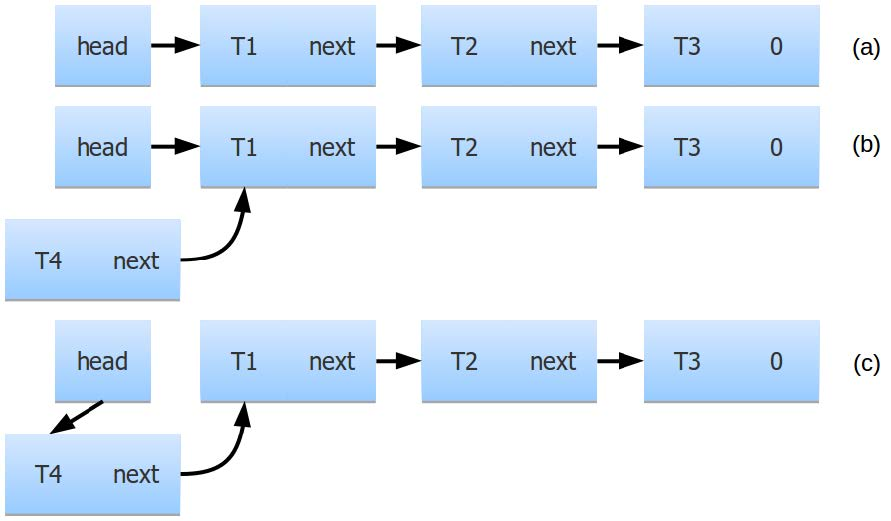
\includegraphics[width=0.9\textwidth]{content/2/chapter7/images/25.jpg}\\
图7.25 - 在单链表的头插入一个新节点
\end{center}

假设我们想在图7.25a所示的列表的头部插入一个新节点。第一步是读取当前头指针,即指向第一个节点的指针。然后用期望值创建新的节点,它的next指针与当前的头指针相同,所以这个节点在当前第一个节点之前链接到链表中(图7.25b)。此时,新节点还不能被任何其他线程访问,因此可以并发地访问数据结构。最后,执行CAS:如果当前头指针没有改变,将用指向新节点的指针替换它(图7.25c)。如果头指针不再具有第一次读取时的值,则读取新值,将其写入新节点的下一个指针,并再次尝试原子CAS。

这是一个简单可靠的算法。这是我们在前一章中看到的发布协议的概括:新数据是在一个线程上创建的,没有考虑线程安全,因为其他线程访问还不能它。作为最后的操作,线程通过原子性地更改可访问所有数据的根指针(我们的例子中是列表的头)来发布数据。如果将新节点插入到另一个节点之后,将自动地更改该节点的next指针。唯一的区别是,多个线程可能试图在同一时间发布新的数据。为了避免数据竞争,我们必须使用\textit{比较和交换}。 

现在,让我们考虑相反的操作,擦除链表的前端节点。这也是通过三个步骤完成的:

%\hspace*{\fill} \\ %插入空行
\begin{center}
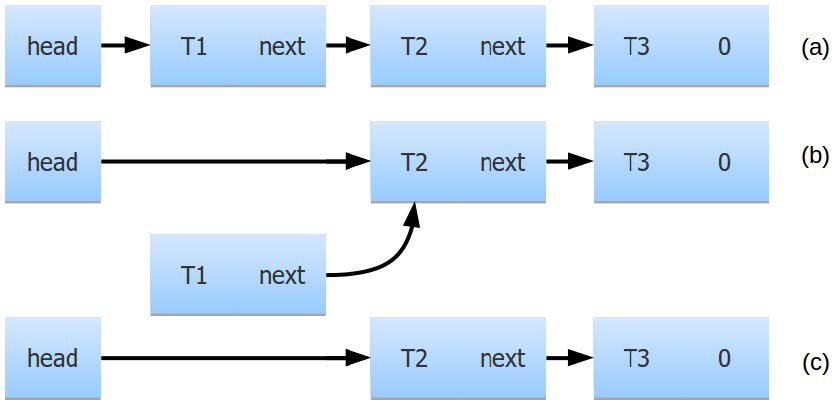
\includegraphics[width=0.9\textwidth]{content/2/chapter7/images/26.jpg}\\
图7.26 - 单链表头部的无锁移除
\end{center}

首先,读取头指针,使用它访问链表的第一个节点,然后读取它的next指针(图7.26a)。然后,我们将next指针的值原子地写入头指针中(图7.26b),但前提是头指针没有改变(CAS)。此时,其他线程访问不能访问前面的第一个节点,这样我们的线程就拥有头指针的原始值,并且可以使用它来删除需要删除的节点(图7.26c)。但是,当我们试图将这两种操作结合起来时,问题就出现了。

让我们假设两个线程同时对链表进行操作,线程A试图删除链表中的第一个节点。第一步是读取头指针和指向next节点的指针,这个指针即将成为列表的新头,但是比较和交换还没有发生。现在,这个头节点是不变的,新头节点是一个值(head'),它只存在于线程A的某个局部变量中。这个时刻如图7.27a所示:

%\hspace*{\fill} \\ %插入空行
\begin{center}
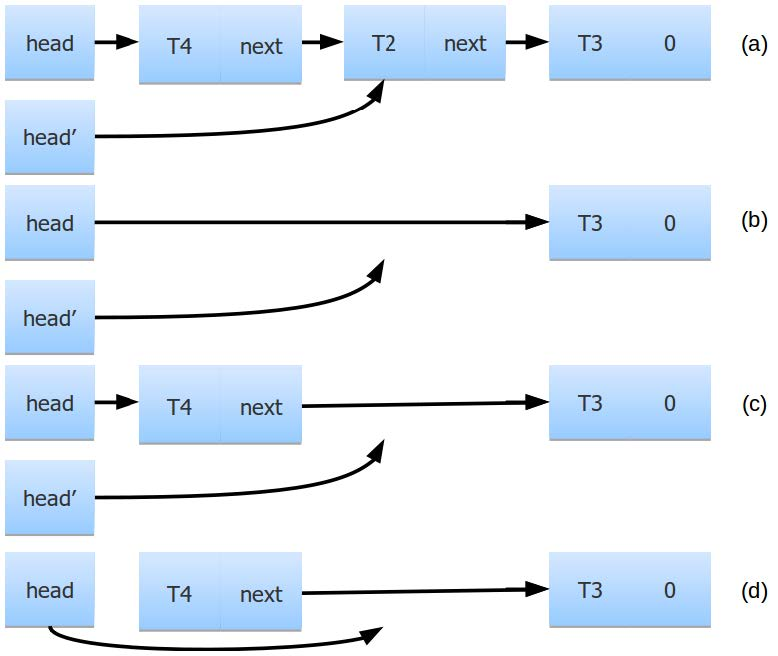
\includegraphics[width=0.9\textwidth]{content/2/chapter7/images/27.jpg}\\
图7.27 - 单链表头部的无锁插入和移除
\end{center}

这时,线程B成功地删除了链表的第一个节点。然后它还会删除下一个节点,使链表保持图7.27b所示的状态(线程A没有取得任何进展)。然后,线程B在链表的开头插入一个新节点(图7.27c)。然而,由于两个已删除节点的内存释放,因此节点T4的新分配重用了之前分配的内存,因此节点T4与原始节点T1拥有了相同的地址。只要删除节点的内存可用于新的分配,这种情况就大概率会发生。事实上,大多数内存分配器更偏爱返回最近释放的内存,前提是它在CPU的缓存中。

现在,线程A终于再次运行了,它要做的操作是比较和交换:如果头指针自线程A上次读取它后没有改变,那么新头成为了现在的头(head')。但是,就线程A所见,头指针的值仍然是相同的(它法观察整个更改历史记录)。CAS操作成功,新的头指针现在指向节点T2以前所使用的内存,而节点T4不再可访问(图7.27d)。自此,整个列表已坏了。

这种故障在无锁数据结构中非常常见,以至于拥有了一个术语:\textbf{A-B-A 问题}。 这里的\textbf{A}和\textbf{B}指的是内存位置:问题是数据结构中的某个指针将其值从A更改为B,然后再返回A。另一个线程只观察初始值和最终值,根本看不到任何更改;比较和交换操作成功,执行的路径是程序员假定数据结构不变的路径。但这个假设是不正确的,数据结构可以任意改变,但没观察到的指针的值的修改,其值就恢复到原来的状态。

The root of the problem is that if the memory is deallocated and reallocated, pointers, or addresses in memory, do not uniquely identify the data stored at that address. There are multiple solutions to this problem, but they all accomplish the same thing by different means: you have to make sure that once you read a pointer that will eventually be used by compare-and-swap, the memory at that address cannot be deallocated until the compare-and-swap is done (successfully or otherwise). If the memory is not deallocated, then another allocation cannot happen at the same address, and you are safe from the A-B-A problem. Note that not deallocating memory is not the same as not deleting nodes: you can certainly make the node inaccessible from the rest of the data structure (remove the node), and you can even call the destructor for the data stored in the node; you just  cannot free the memory occupied by the node. 

There are many ways to solve the A-B-A problem by delaying memory deallocation. The application-specific options are usually the simplest if they are possible. If you know that the algorithm does not remove many nodes over the lifetime of the data structure, you may simply keep all removed nodes on a list of deferred deallocations, to be deleted when the entire data structure is deleted. A more general version of this approach can be described as application-driven garbage collection: all deallocated memory goes on a garbage list first. The garbage memory is periodically returned to the main memory allocator, but during this garbage collection, all operations on the data structure are suspended: the operations in progress must complete before the collection starts, and all new operations are blocked until the collection is done. This ensures that no compare-and-swap operation can span the time interval of the garbage collection and, thus, the recycled memory is never encountered by any operation. The popular and often very efficient RCU (read-copy-update) technique is a variant of this method as well. Another common approach is the use of hazard pointers.

In this book, we will present yet another approach that employs atomic shared pointers (std::shared\_ptr is not atomic by itself, but the standard included the necessary functions for atomic operations on shared pointers, or you can write your own for this specific application and make it faster). Let's revisit Figure 7.27b, but now let all pointers be atomic shared pointers. As long as there is at least one such pointer to a node, that node cannot be deallocated. In the same sequence of events, thread A still has the old head pointer that points to the original node T1, as well as the intended new head pointer, head', that points to the node T2. 

%\hspace*{\fill} \\ %插入空行
\begin{center}
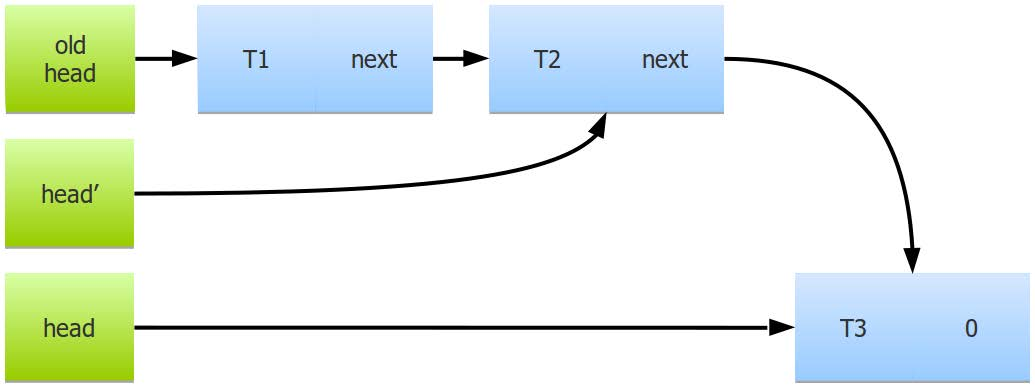
\includegraphics[width=0.9\textwidth]{content/2/chapter7/images/28.jpg}\\
Figure 7.28 – Lock-free insertion and removal at the head of a singly-linked list with shared pointers
\end{center}

Thread B has removed both nodes from the list (Figure 7.28), but the memory has not been released. The new node T4 is allocated at some other address, different from the addresses of all currently allocated nodes. Thus, when thread A resumes execution, it will find the new list head different from the old head value; the compare-and-swap will fail, and thread A will attempt the operation again. At this point, it will re-read the head pointer (and get the address of the node T3). The old value of the head pointer is now gone; since it was the last shared pointer pointing to the node T1, this node has no more references and is deleted. Similarly, node T2 is deleted as soon as the shared pointer head' is reset to its new intended value (the next pointer of the node T3). Both nodes T1 and T2 have no shared pointers pointing to them, so they are finally deleted. 

Of course, this takes care of the insertion at the front. To allow insertion and removal anywhere, we have to make all pointers to the nodes into shared pointers. This includes the next pointers of all nodes as well as the pointers to nodes that are hidden inside list iterators. Such a design has another major advantage: it takes care of the problems with list traversals (such as search operations) that happen concurrently with insertions and deletions.

If a list node was removed while there is an iterator pointing to this list (Figure 7.29), the node remains allocated, and the iterator is valid. Even if we remove the next node (T3), it will not be deallocated because there is a shared pointer pointing to it (the next pointer of node T2). The iterator can traverse the entire list.

%\hspace*{\fill} \\ %插入空行
\begin{center}
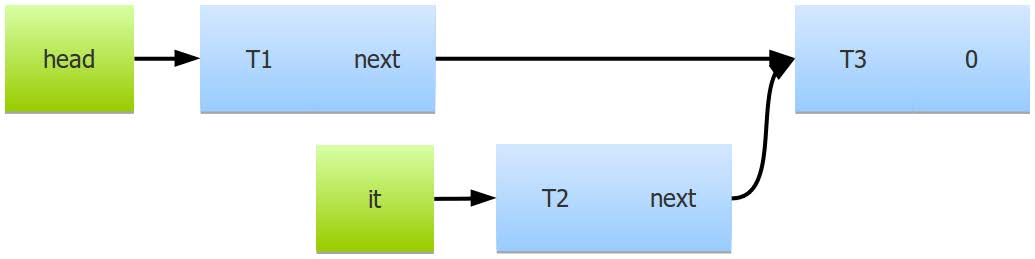
\includegraphics[width=0.9\textwidth]{content/2/chapter7/images/29.jpg}\\
Figure 7.29 – Thread-safe traversal of a lock-free list with atomic shared pointers
\end{center}

Of course, this traversal may include nodes that are no longer in the list, that is, no longer reachable from the head of the list. This is the nature of the concurrent data structures: there is no meaningful way to talk about the current content of the list: the only way to know the content of the list is to iterate over it from the head to the last node, but, by the time the iterator reached the end of the list, the previous nodes might have changed, and the result of the traversal is no longer current. This way of thinking takes some getting used to. 

We are not going to show any benchmarks of the lock-free list versus a lock-guarded list because these benchmarks must be specific to the application. If you benchmark only insertions and deletions at the head of the list (push\_front() and pop\_front()), the spinlock-guarded list will be faster (atomic shared pointers are not cheap). On the other hand, if you benchmark simultaneous insertions and searches, you can make the lock-free list faster by as much as you want: do a traversal of a list of 1M elements with the lock-guarded list locked the entire time while the lock-free list can do simultaneous iterations on every thread, along with insertions and deletions. No matter how slow the atomic pointers are, the lock-free list will be faster if you just make it long enough. This is not a gratuitous observation: your application may need to do the operations that would require locking the list for a very long time unless you can somehow partition the list in a way that avoids deadlocks. If this is what you need to do, the lock-free list is the fastest by far. On the other hand, if you need to iterate over just a few elements and never in many different locations at the same time, a lock-guarded list will do fine. 

The A-B-A problem and the solutions we have listed apply not just to the lists but to all nodal data structures: doubly-linked list, tree, and graph. In data structures linked by multiple pointers, you may encounter additional problems. First of all, even if all pointers are atomic, changing two atomic pointers one after the other is not an atomic operation. This leads to temporary inconsistencies in the data structure: for example, you may expect that going from a node to the next node and back to the previous node will get you back to the original node. This is not always true in the case of concurrency: if a node is inserted or removed at this location, one of the pointers may be updated before the other. The second problem is specific to shared pointers or any other implementation that uses reference counting: if the data structure has pointer loops, the nodes in the loop do not get deleted even when there are no more external references to them. The simplest example is the doubly-linked list, where two adjacent nodes always have pointers to each other. The way we solve this problem in single-threaded programs is by using weak pointers (in a doubly-linked list, all next pointers could be shared, and all previous pointers would then be weak). This does not work as well for concurrent programs: the whole point is to delay the deallocation of memory until there are no more references to it, and the weak pointers do not do that. For these cases, additional garbage collection may be necessary: after the last external pointer to a node is deleted, we have to traverse the linked nodes and check whether there are any external pointers to them (we can do it by checking the reference counts). List fragments with no external pointers can be safely deleted. For such data structures, alternative approaches such as hazard pointers or explicit garbage collection may be preferred. The reader should refer to specialized publications on lock-free programming for more information on these methods. 

This concludes our exploration of high-performance data structures for concurrent programming. Let's now summarize what we have learned.













